\clearpage
\section{\texorpdfstring{\underline{Search and Analysis}}{Search and Analysis}}

\clearpage
\section{\texorpdfstring{\underline{Data Structures}}{Data Structures}}
\subsection{Trees}
\subsubsection{Basic Tree Terminology}
\textbf{Height:} The height of a tree is the length of the longest path from the root to a leaf. It is the number of edges on this path.

\textbf{Level:} The level of a node is the number of edges on the path from the root to the node. The root node is at level 0.

\textbf{Minimum Width:} The minimum width of a tree is the smallest number of nodes at any level of the tree.

\textbf{Maximum Width:} The maximum width of a tree is the largest number of nodes at any level of the tree.

\textbf{Depth:} The depth of a node is the number of edges from the node to the tree's root node.

\textbf{Leaf:} A leaf is a node with no children.

\textbf{Internal Node:} An internal node is a node with at least one child.

\textbf{Binary Tree:} A tree data structure in which each node has at most two children, referred to as the left child and the right child.

\subsubsection{KD-Trees}
\textbf{Problem Type:} Construction of a KD-Tree from 2D points

\textbf{What to Look For:}
\begin{itemize}[noitemsep,leftmargin=*]
    \item Set of 2D points given as coordinates
    \item Request to build a KD-Tree
    \item Questions about tree properties (height, leaves)
\end{itemize}

\textbf{Given Points:} 
$P = \{(1,3), (12,1), (4,5), (5,4),$ \\
\hspace*{1cm} $(10,11), (8,2), (2,7)\}$

\textbf{Solution Strategy:}
\begin{enumerate}[leftmargin=*,noitemsep]
    \item Sort points by x-coordinate (root level)
    \item Find median point
    \item Split into left/right subtrees
    \item Repeat with y-coordinates for next level
    \item Continue alternating x/y until all points placed
\end{enumerate}

\textbf{Detailed Solution:}
\begin{enumerate}[leftmargin=*,label=\arabic*.]
    \item \textbf{Root Level (x-split)}
    \begin{itemize}[noitemsep]
        \item Sorted x: \\
        $(1,3), (2,7), (4,5),$ \\
        $\mathbf{(5,4)},$ \\
        $(8,2), (10,11), (12,1)$
        \item Median $(5,4)$ becomes root $\ell_1$
    \end{itemize}

    \begin{figure}[H]
    \centering
    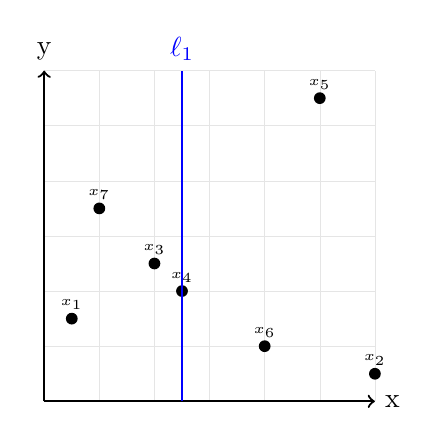
\begin{tikzpicture}[scale=0.35]
        % Grid
        \draw[very thin,gray!20] (0,0) grid[step=2] (12,12);
        \draw[->,thick] (0,0) -- (12,0) node[right] {x};
        \draw[->,thick] (0,0) -- (0,12) node[above] {y};
        
        % Points with labels
        \foreach \x/\y/\label in {
            1/3/1, 12/1/2, 4/5/3, 5/4/4, 10/11/5, 8/2/6, 2/7/7
        } {
            \node[circle,fill,inner sep=1.5pt] at (\x,\y) {};
            \node[font=\tiny] at (\x,\y+0.5) {$x_{\label}$};
        }
        
        % Splitting line
        \draw[blue,thick] (5,0) -- (5,12) node[above] {$\ell_1$};
    \end{tikzpicture}
    \caption*{Coordinate Split at Root Level}
    \end{figure}

    \item \textbf{Tree Structure}
    \begin{figure}[H]
    \centering
    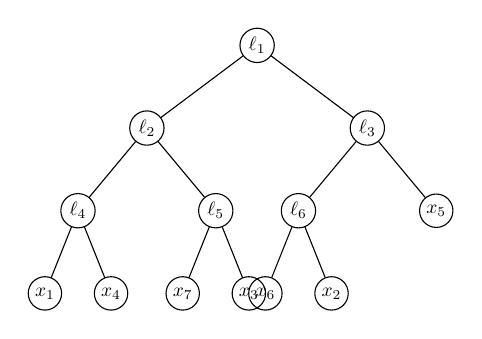
\begin{tikzpicture}[
        level distance=1.5cm,
        level 1/.style={sibling distance=4cm},
        level 2/.style={sibling distance=2.5cm},
        level 3/.style={sibling distance=1.2cm},
        scale=0.7,
        every node/.style={transform shape}
    ]
    \node [circle,draw,inner sep=2pt] {$\ell_1$}
        child {node [circle,draw,inner sep=2pt] {$\ell_2$}
            child {node [circle,draw,inner sep=2pt] {$\ell_4$}
                child {node [circle,draw,inner sep=2pt] {$x_1$}}
                child {node [circle,draw,inner sep=2pt] {$x_4$}}
            }
            child {node [circle,draw,inner sep=2pt] {$\ell_5$}
                child {node [circle,draw,inner sep=2pt] {$x_7$}}
                child {node [circle,draw,inner sep=2pt] {$x_3$}}
            }
        }
        child {node [circle,draw,inner sep=2pt] {$\ell_3$}
            child {node [circle,draw,inner sep=2pt] {$\ell_6$}
                child {node [circle,draw,inner sep=2pt] {$x_6$}}
                child {node [circle,draw,inner sep=2pt] {$x_2$}}
            }
            child {node [circle,draw,inner sep=2pt] {$x_5$}}
        };
    \end{tikzpicture}
    \caption*{KD-Tree Structure}
    \end{figure}
    \FloatBarrier

    \item \textbf{Final Properties}
    \begin{itemize}[noitemsep,leftmargin=*]
        \item Height: 3 (counting from 0)
        \item Leaves: 7 (all original points)
        \item Second leaf from left: $(4,5)$
    \end{itemize}
\end{enumerate}

\textbf{Exam Tips:}
\begin{enumerate}[noitemsep,leftmargin=*]
    \item Always start by sorting points on current dimension
    \item Mark median point clearly in your sorting
    \item Draw coordinate system with splitting lines
    \item Keep track of which dimension you're splitting on:
        \begin{itemize}[noitemsep,topsep=0pt]
            \item Level 0: x-coordinate
            \item Level 1: y-coordinate
            \item Level 2: x-coordinate
            \item And so on...
        \end{itemize}
    \item Verify tree properties at the end
\end{enumerate}

\textbf{Common Mistakes to Avoid:}
\begin{itemize}[noitemsep,leftmargin=*]
    \item Don't forget to alternate dimensions
    \item Don't skip sorting at each level
    \item Don't mix up left (<) and right (>) subtrees
    \item Don't forget to verify final tree properties
\end{itemize}

\FloatBarrier

\subsubsection{KD-Tree Complexity Analysis}
\textbf{Problem Type:} Complexity proof for KD-Tree construction

\textbf{What to Look For:}
\begin{itemize}[noitemsep,leftmargin=*]
    \item Proof of time complexity $O(n\log n)$
    \item Proof of space complexity $O(n)$
    \item Recursive analysis
\end{itemize}

\textbf{Solution Strategy:}
\begin{enumerate}[leftmargin=*,noitemsep]
    \item Prove space complexity first (easier)
    \item Analyze recursive structure
    \item Set up recurrence relation
    \item Apply Master Theorem
\end{enumerate}

\textbf{Space Complexity Proof:}
\begin{enumerate}[leftmargin=*,noitemsep]
    \item For $n = 2^k$ points:
        \begin{itemize}[noitemsep,topsep=0pt]
            \item Internal nodes (parents): $2^k - 1$
            \item Total nodes: $2^k + 2^{k-1} = n + n/2 = 3n/2 < 3n$
        \end{itemize}
    \item For general $n$ (not power of 2):
        \begin{itemize}[noitemsep,topsep=0pt]
            \item Find $t$ where $2^{t-1} < n < 2^t$
            \item Internal nodes $n_p$: $2^{t-2} < n_p < 2^{t-1}$
            \item Total nodes: $3 \cdot 2^{t-2} < n + n_p < 3 \cdot 2^{t-1}$
            \item Therefore: $n + n_p < 3n$
        \end{itemize}
    \item Each node uses $O(1)$ storage
    \item Total storage: $O(1) \cdot O(n) = O(n)$
\end{enumerate}

\textbf{Time Complexity Proof:}
\begin{enumerate}[leftmargin=*,noitemsep]
    \item At each recursion:
        \begin{itemize}[noitemsep,topsep=0pt]
            \item Split $n$ points into two subsets of $n/2$
            \item Finding median costs $O(n)$
        \end{itemize}
    \item Recurrence relation:
        \[ T(n) = \begin{cases}
            O(1) & \text{if } n = 1 \\
            2T(n/2) + O(n) & \text{if } n > 1
        \end{cases} \]
    \item Apply Master Theorem:
        \begin{itemize}[noitemsep,topsep=0pt]
            \item Similar to Merge-Sort analysis
            \item Results in $T(n) = O(n\log n)$
        \end{itemize}
\end{enumerate}

\textbf{Key Points for Exam:}
\begin{itemize}[noitemsep,leftmargin=*]
    \item Space complexity proof:
        \begin{itemize}[noitemsep,topsep=0pt]
            \item Count nodes for power of 2
            \item Extend to general case
            \item Multiply by constant storage
        \end{itemize}
    \item Time complexity proof:
        \begin{itemize}[noitemsep,topsep=0pt]
            \item Identify recursive pattern
            \item Write recurrence relation
            \item Apply Master Theorem
        \end{itemize}
    \item Remember median finding is $O(n)$
\end{itemize}

\textbf{Common Mistakes to Avoid:}
\begin{itemize}[noitemsep,leftmargin=*]
    \item Don't forget to account for non-power-of-2 cases
    \item Don't ignore constant factors in space analysis
    \item Remember to justify linear median finding
    \item Don't skip the Master Theorem application
\end{itemize}

\FloatBarrier

\subsubsection{Binary Search Trees (BST)}
\textbf{Definition:} A binary tree where for each node $x$:
\begin{itemize}[noitemsep,leftmargin=*]
    \item All keys in left subtree are < $x.key$
    \item All keys in right subtree are > $x.key$
    \item No duplicate keys allowed
\end{itemize}

\textbf{Basic Operations:}
\begin{enumerate}[noitemsep,leftmargin=*]
    \item \textbf{TREE-SEARCH$(x,k)$}: Find node with key $k$
        \begin{itemize}[noitemsep,topsep=0pt]
            \item Start at root, compare with $k$
            \item If equal: found
            \item If $k$ smaller: go left
            \item If $k$ larger: go right
            \item Time: $O(h)$ where $h$ is height
        \end{itemize}
    
    \item \textbf{TREE-MINIMUM$(x)$}: Find smallest key
        \begin{itemize}[noitemsep,topsep=0pt]
            \item Follow left pointers until NIL
            \item Time: $O(h)$
        \end{itemize}
    
    \item \textbf{TREE-MAXIMUM$(x)$}: Find largest key
        \begin{itemize}[noitemsep,topsep=0pt]
            \item Follow right pointers until NIL
            \item Time: $O(h)$
        \end{itemize}
    
    \item \textbf{TREE-SUCCESSOR$(x)$}: Find next larger key
        \begin{itemize}[noitemsep,topsep=0pt]
            \item If right subtree exists: TREE-MINIMUM(right)
            \item Else: Go up until first right turn
            \item Time: $O(h)$
        \end{itemize}
    
    \item \textbf{TREE-PREDECESSOR$(x)$}: Find next smaller key
        \begin{itemize}[noitemsep,topsep=0pt]
            \item If left subtree exists: TREE-MAXIMUM(left)
            \item Else: Go up until first left turn
            \item Time: $O(h)$
        \end{itemize}
\end{enumerate}

\textbf{Modifying Operations:}
\begin{enumerate}[noitemsep,leftmargin=*]
    \item \textbf{TREE-INSERT$(T,z)$}: Insert new node $z$
        \begin{itemize}[noitemsep,topsep=0pt]
            \item Follow BST property down to leaf
            \item Insert as left/right child
            \item Time: $O(h)$
        \end{itemize}
    
    \item \textbf{TREE-DELETE$(T,z)$}: Delete node $z$
        \begin{itemize}[noitemsep,topsep=0pt]
            \item Case 1: No children - remove directly
            \item Case 2: One child - replace with child
            \item Case 3: Two children:
                \begin{itemize}[noitemsep,topsep=0pt]
                    \item Find successor $y$ (min in right subtree)
                    \item Replace $z$ with $y$
                    \item Delete $y$ from original position
                \end{itemize}
            \item Time: $O(h)$
        \end{itemize}
\end{enumerate}

\textbf{Helper Operation:}
\begin{itemize}[noitemsep,leftmargin=*]
    \item \textbf{TRANSPLANT$(T,u,v)$}: Replace subtree
        \begin{itemize}[noitemsep,topsep=0pt]
            \item Replaces subtree rooted at $u$ with subtree rooted at $v$
            \item Updates parent pointers
            \item Used in DELETE operation
        \end{itemize}
\end{itemize}

\textbf{Properties:}
\begin{itemize}[noitemsep,leftmargin=*]
    \item Inorder traversal gives sorted sequence
    \item Height $h$ determines operation time:
        \begin{itemize}[noitemsep,topsep=0pt]
            \item Best case (balanced): $h = \lg n$
            \item Worst case (linear): $h = n$
        \end{itemize}
    \item No explicit balancing - shape depends on insertion order
\end{itemize}

\textbf{Tree Traversal:}
\begin{itemize}[noitemsep,leftmargin=*]
    \item \textbf{Inorder}: Left subtree → Root → Right subtree
        \begin{itemize}[noitemsep,topsep=0pt]
            \item Visits nodes in sorted order
            \item Used for ordered printing
        \end{itemize}
    \item \textbf{Preorder}: Root → Left subtree → Right subtree
        \begin{itemize}[noitemsep,topsep=0pt]
            \item Root processed before children
            \item Used for copying tree structure
        \end{itemize}
    \item \textbf{Postorder}: Left subtree → Right subtree → Root
        \begin{itemize}[noitemsep,topsep=0pt]
            \item Root processed after children
            \item Used for deletion
        \end{itemize}
\end{itemize}

\textbf{Implementation Details:}
\begin{itemize}[noitemsep,leftmargin=*]
    \item Node structure:
        \begin{itemize}[noitemsep,topsep=0pt]
            \item key: Value stored in node
            \item left, right: Pointers to children
            \item p: Pointer to parent (optional)
        \end{itemize}
    \item Sentinel NIL:
        \begin{itemize}[noitemsep,topsep=0pt]
            \item Used to mark leaf nodes
            \item Simplifies boundary conditions
        \end{itemize}
\end{itemize}

\textbf{Key Insights:}
\begin{itemize}[noitemsep,leftmargin=*]
    \item Successor never has left child
    \item Predecessor never has right child
    \item All operations maintain BST property
    \item Performance depends on tree height
    \item Balancing requires additional mechanisms (AVL, Red-Black)
\end{itemize}

\clearpage
\section{\texorpdfstring{\underline{Complexity Analysis}}{Complexity Analysis}}

\subsection{Sorting Complexity}
\textbf{Big-Oh Notation:} Describes the upper bound of an algorithm's running time. For example, $O(n \log n)$ is common in efficient sorting algorithms like Merge Sort.

\subsection{Quadratic Algorithms}
\textbf{Understanding $O(n^2)$:} Often seen in simple sorting algorithms like Bubble Sort, where each element is compared to every other element.

\subsection{Time Complexity}
\textbf{Complexity Classes:} Includes constant $O(1)$, logarithmic $O(\log n)$, linear $O(n)$, quadratic $O(n^2)$, and more. Helps in understanding the efficiency of algorithms.

\subsection{Dominant Terms}
\textbf{Identifying Dominant Terms:} In expressions like $5n^2 + 3n \log n$, the term $5n^2$ is dominant, leading to $O(n^2)$.

\subsection{Big-Oh Notation Properties}
\textbf{Rules:} Includes the rule of sums $O(f + g) = O(\max\{f, g\})$ and products $O(f \cdot g) = O(f) \cdot O(g)$.

\subsection{Computational Complexity}
\textbf{Nested Loops:} Analyzing loops within loops to determine total complexity, such as $O(n(\log n)^2)$ for certain nested structures.

\subsection{Master Theorem}
The Master Theorem provides a way to solve recurrence relations of the form:

\[ T(n) = aT\left(\frac{n}{b}\right) + f(n) \]

where $a \geq 1$, $b > 1$, and $f(n)$ is an asymptotically positive function. The theorem helps determine the asymptotic behavior of $T(n)$ by comparing $f(n)$ with $n^{\log_b a}$:

1. If $f(n) = O(n^{\log_b a - \epsilon})$ for some $\epsilon > 0$, then:
   \[ T(n) = \Theta(n^{\log_b a}) \]

2. If $f(n) = \Theta(n^{\log_b a})$, then:
   \[ T(n) = \Theta(n^{\log_b a} \log n) \]

3. If $f(n) = \Omega(n^{\log_b a + \epsilon})$ for some $\epsilon > 0$, and if $af(n/b) \leq cf(n)$ for some constant $c < 1$ and sufficiently large $n$, then:
   \[ T(n) = \Theta(f(n)) \]

The Master Theorem is widely used in analyzing the time complexity of divide-and-conquer algorithms, such as Merge Sort and Quick Sort.

\subsection{Heap Operations}
\textbf{Basic Heap Properties:}
\begin{itemize}
    \item A heap is a complete binary tree
    \item In a max-heap, for each node $i$: parent.key $\geq$ children.key
    \item In a min-heap, for each node $i$: parent.key $\leq$ children.key
\end{itemize}

\textbf{Array Representation:}
For a node at index $i$:
\begin{itemize}
    \item Parent: $\lfloor i/2 \rfloor$
    \item Left child: $2i$
    \item Right child: $2i + 1$
\end{itemize}

\begin{figure}[H]
    \centering
    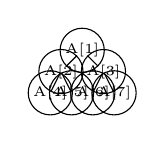
\begin{tikzpicture}[scale=0.45,
        level distance=0.6cm,
        level 1/.style={sibling distance=1.2cm},
        level 2/.style={sibling distance=0.6cm},
        every node/.style={circle,draw,inner sep=1pt,font=\tiny}]
        \node {A[1]}
            child {node {A[2]}
                child {node {A[4]}}
                child {node {A[5]}}
            }
            child {node {A[3]}
                child {node {A[6]}}
                child {node {A[7]}}
            };
    \end{tikzpicture}
    \caption*{\footnotesize Array indices in heap}
\end{figure}

\textbf{MAX-HEAPIFY Operation:}
\begin{enumerate}
    \item Compare root with children
    \item If child is larger, swap with largest child
    \item Recursively heapify affected subtree
\end{enumerate}

\begin{figure}[H]
    \centering
    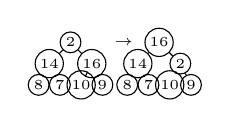
\begin{tikzpicture}[scale=0.45,
        level distance=0.6cm,
        level 1/.style={sibling distance=1.2cm},
        level 2/.style={sibling distance=0.6cm},
        every node/.style={circle,draw,inner sep=1pt,font=\tiny}]
        % Before MAX-HEAPIFY
        \node {2}
            child {node {14}
                child {node {8}}
                child {node {7}}
            }
            child {node {16}
                child {node {10}}
                child {node {9}}
            };
            
        % Arrow
        \node[draw=none] at (1.5,0) {$\rightarrow$};
        
        % After MAX-HEAPIFY
        \begin{scope}[xshift=2.5cm]
        \node {16}
            child {node {14}
                child {node {8}}
                child {node {7}}
            }
            child {node {2}
                child {node {10}}
                child {node {9}}
            };
        \end{scope}
    \end{tikzpicture}
    \caption*{\footnotesize MAX-HEAPIFY example}
\end{figure}

\textbf{BUILD-MAX-HEAP Operation:}
\begin{enumerate}
    \item Start from last non-leaf node ($\lfloor n/2 \rfloor$)
    \item Apply MAX-HEAPIFY to each node up to root
\end{enumerate}

\begin{figure}[H]
    \centering
    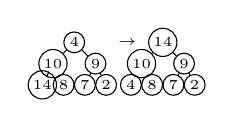
\begin{tikzpicture}[scale=0.45,
        level distance=0.6cm,
        level 1/.style={sibling distance=1.2cm},
        level 2/.style={sibling distance=0.6cm},
        every node/.style={circle,draw,inner sep=1pt,font=\tiny}]
        % Initial array as tree
        \node {4}
            child {node {10}
                child {node {14}}
                child {node {8}}
            }
            child {node {9}
                child {node {7}}
                child {node {2}}
            };
            
        % Arrow
        \node[draw=none] at (1.5,0) {$\rightarrow$};
        
        % After BUILD-MAX-HEAP
        \begin{scope}[xshift=2.5cm]
        \node {14}
            child {node {10}
                child {node {4}}
                child {node {8}}
            }
            child {node {9}
                child {node {7}}
                child {node {2}}
            };
        \end{scope}
    \end{tikzpicture}
    \caption*{\footnotesize BUILD-MAX-HEAP example}
\end{figure}

\textbf{HEAPSORT Operation:}
\begin{enumerate}
    \item BUILD-MAX-HEAP
    \item Repeatedly:
        \begin{itemize}[noitemsep,topsep=0pt]
            \item Swap root with last element
            \item Reduce heap size by 1
            \item MAX-HEAPIFY root
        \end{itemize}
\end{enumerate}
